\subsection{Популярность}

Результаты сравнения популярности приведены в таблице \ref{tab:popularity-comparison}.

\begin{table}[h!]
    \centering
    \begin{tabular}{lccc}
        \toprule
        \textbf{Фреймворк} & \textbf{Количество проектов} & \textbf{Количество звезд} \\
        \midrule
        EML & 258 & - \\
        MLX & 61 & 123 \\
        TYXML & 1200+ & 173 \\
        DHTML & 20 & 181 \\
        \bottomrule
    \end{tabular}
    \caption{Сравнение популярности}
    \label{tab:popularity-comparison}
\end{table}

Результаты сравнения (Таблица~\ref{tab:popularity-comparison}) демонстрируют парадоксальную ситуацию: фреймворки с максимальной распространённостью в реальных проектах (TYXML) имеют относительно низкие показатели интереса сообщества (GitHub звезды), тогда как менее используемые решения (DHTML) демонстрируют обратную динамику.
Этот феномен хорошо иллюстрирует известный тезис Б. Страуструпа:
\begin{quote}
    «Есть только два вида языков: те, на которые всё время жалуются, и те, которыми никто не использует» \cite{two_kinds}.
\end{quote}

Перенеся эту логику на шаблонизаторы, можно выделить:
\begin{itemize}
    \item \textbf{TYXML} — попадает в первую категорию: активное использование (1200+ проектов) сопровождается умеренным интересом сообщества (173 звезд), что типично для зрелых решений с известными ограничениями
    \item \textbf{MLX} — относятся ко второй группе: минимальное количество использований (258 и 61 проект) при полном отсутствии "звёздной" популярности, что свидетельствует о фундаментальных барьерах для внедрения
    \item \textbf{DHTML} — занимает промежуточное положение: низкое промышленное применение (20 проектов) при относительно высоком маркетинговом потенциале (181 звезда), характерное для нишевых экспериментальных инструментов
\end{itemize}

\subsection{Покрытие}

Визуальное сравнение приведено в приложении \ref{apx:coverage}.
Его результаты таковы:

\begin{table}[h]
    \centering
    \caption{Сравнение покрытия}
    \label{tab:coverage-comparison}
    \begin{tabularx}{\linewidth}{l>{\raggedright\arraybackslash}X>{\raggedright\arraybackslash}XcXX}
        \toprule
        \textbf{Фреймворк} & \textbf{Комментарии} \\
        \midrule
        EML & \cellcolor{yellow!30} Изначальный шаблон теряется после работы препроцессора, результирующий код нечитабелен \\
        MLX & После препроцессора шаблон трансформируется в корректный OCaml код \\
        TYXML, DHTML & Не используется препроцессор, оригинальный код покрывается без потерь \\
        TYXML\% & Препроцессор в этом случае генерирует AST, которое в свою очередь обходится bisect-ом. Оригинальное представление кода сохраняется в покрытии \\
        \bottomrule
    \end{tabularx}
\end{table}

Как видно из сравнения, EML сильно проигрывает остальным шаблонизаторам, полностью теряя оригинальную структуру кода.

\subsection{Экосистема}

Результаты исследования приведены в таблице \ref{tab:ecosystem}.
Сниппетов не существует ни для одного из этих фреймворков, поэтому эта колонна исключена из сравнения.

\begin{table}[h!]
    \begin{tabularx}{\linewidth}{l>{\raggedright\arraybackslash}X>{\raggedright\arraybackslash}XcXX}
        \toprule
        \textbf{Фреймворк} & \textbf{Подсветка} \\
        \midrule
        EML & \cellcolor{yellow!30} Подсветки нет \\
        MLX & Была добавлена в мае 2025 с версией VSCode OCaml platform 1.30.0 \\
        TyXML, DHTML & Подсветка OCaml \\
        TyXML\% & Подсветка OCaml. Однако, синтаксис на основе let\%, будучи основанным на строковом представлении, не подсвечивается, как и допущенные ошибки. Обновление происходит только после перезапуска компиляции \\
        \bottomrule
    \end{tabularx}
    \caption{Обзор экосистемы фреймворков}
    \label{tab:ecosystem}
\end{table}

Подсветка EML полностью отсутствует.
Это связано с природой EML - будучи строковым парсером, описание грамматики крайне сложно.

Напротив, совсем недавно появилась подсветка для MLX, как раз реализующая такой подход.
Стоит также отметить что в случае MLX это удалось сделать так как правила разделения OCaml и HTML кода в нем являются значительно более простыми и менее вариативными.


\subsection{Документация}

\begin{table}[h!]
\begin{tabularx}{\textwidth}{
    lXXXXX}
    \toprule
 & EML & MLX & TyXML & TyXML\% & DHTML \\
 \midrule
Экосистема & Правило для dune & Примеры интеграции & Пакет OCaml & Пример интеграции & Пакет OCaml \\

Работа & Есть примеры & + &  &  &  \\
Принцип & - & + & \multicolumn{2}{l}{} &  \\
Актуальность & + & +/-\ref{com:mlx} & \multicolumn{2}{l}{+} & + \\
Корректность & + & + &  &  & + \\
Полнота & + & - &  &  & + \\
Удобство & Сайт & README & \multicolumn{2}{l}{} & + \\
\bottomrule
\end{tabularx}
\caption{Сравнение документаций}
\label{tab:docs}
\end{table}

\begin{minipage}{.8\linewidth}
\footnotesize
\textbf{Комментарии:}
\begin{enumerate}
    \item \label{com:eml}
    Низкая производительность обусловлена строковыми операциями. 
    Преимущество интеграции - входит в состав Dream. 
    Планируется оптимизация через кэширование AST.
    
    \item \label{com:tyxml}
    Лучшая безопасность за счёт статической типизации. 
    Сложность интеграции с новыми инструментами требует ручной настройки.
    
    \item \label{com:mlx}
    Указано что поддержки подсветки еще нет, однако это неправда
    Проблемы интеграции вызваны зависимостью от JSX-транслятора. 
    Производительность улучшена в последнем релизе v0.3.
\end{enumerate}
\end{minipage}

\subsection{Поддержка UTF-8}

Все фреймворки поддерживают UTF-8.
Примеры приведены на рис. \ref{fig:utf8}.

После препроцессинга (для EML и MLX) русские символы заменяются их экранированным представлением в UTF-8.
Результирующие строки корректны в OCaml, однако нечитабельны без инструментов.
Эта проблема важна только при чтении покрытия или сгенерированного кода, тогда как генерируемые HTML страницы полностью корректны.

В случае TyXML\% первый символ просто неправильно отображается в сгенерированном покрытии, хотя код страницы получающийся в результате работы функции корректен.
В связи с этим, сделан вывод что это ошибка на стороне bisect\_ppx и дальнешее исследование не было проделано.

\begin{figure}[ht!]
    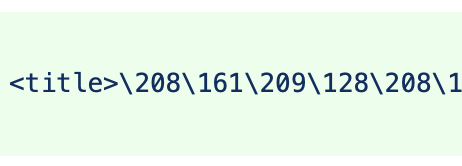
\includegraphics[width=.3\textwidth]{utf8eml}\hfill
    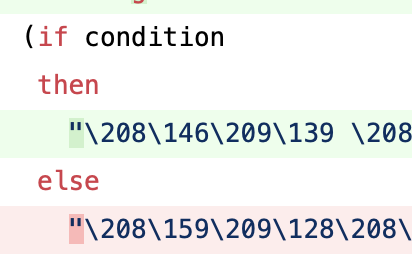
\includegraphics[width=.3\textwidth]{utf8mlx}\hfill
    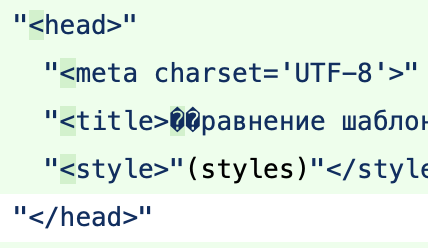
\includegraphics[width=.3\textwidth]{utf8tyxml}
    \caption{EML, экранированные UTF-8 символы}
    \caption{MLX, экранированные UTF-8 символы}
    \caption{TyXML, ошибка отображения первых символов в строке}
    \label{fig:utf8}
\end{figure}
